% --
% intro

\section{Introduction}
\sectionheader{Introduction}

\begin{frame}
  \frametitle{KWS Game Pipeline}
  \begin{figure} 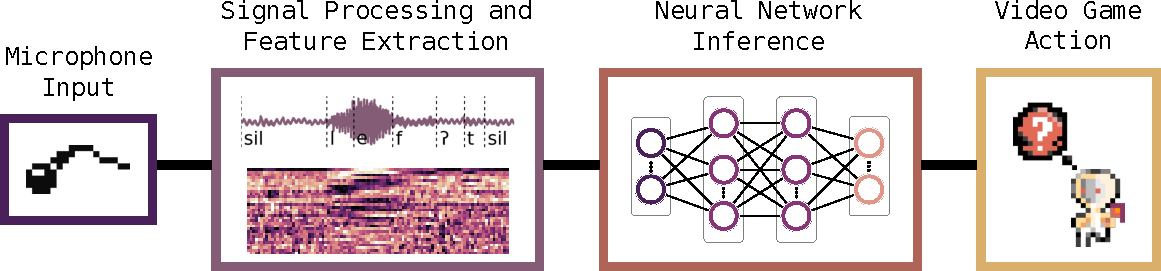
\includegraphics[width=0.9\textwidth]{../1_intro/figs/intro_kws.pdf} \end{figure}
  \scriptsize
  \vspace{0.3cm}
  \centering
  \begin{tikzpicture}[opacity=0.6]
    \node at (0, 0) (level) {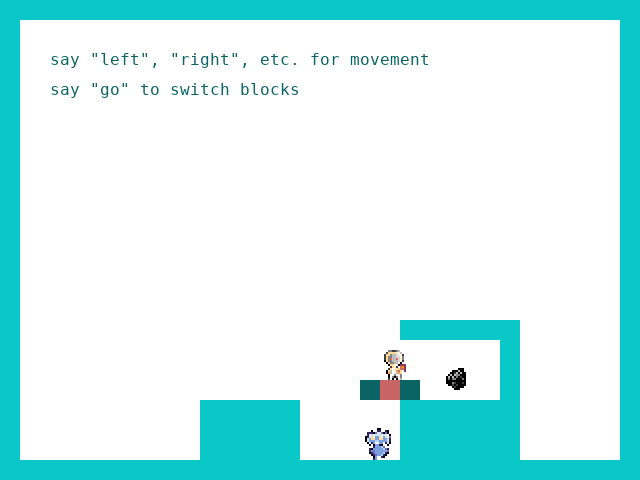
\includegraphics[width=0.25\textwidth]{../../screenshots/level1-2.png}};
    \node at (level.south) [anchor=north] {watch the intro video...};
    \node at (level.center) (tri) [circle, fill=black!25, inner sep=3mm, opacity=1.0] {};
    \begin{scope}[scale=0.5]
      \fill [color=white, opacity=1.0, yshift=-0.5cm, xshift=-0.34cm] (0, 0) -- (0, 1) -- (0.85, 0.5) -- cycle;
    \end{scope}
  \end{tikzpicture}
\end{frame}

\begin{frame}
  \frametitle{KWS Problem Formulation}
  \begin{itemize}
    \item vocabulary with $L$ words:
    \begin{equation*}\label{eq:intro_kws_dict}
      S \coloneqq \{s_i \mid i = 0, 1, \dots, L - 1\},
    \end{equation*}

    \item closest word for target word $t$:
    \begin{equation*}\label{eq:intro_kws_task}
      \hat{s} = \underset{s_i \in S}{\arg \min} \, \mathcal{D}(t, s_i),
    \end{equation*}

    \item word prediction with neural network outputs $y_i$:
    \begin{equation*}\label{eq:intro_kws_class}
      \hat{s} = s_{\underset{i = 0, 1, \dots, L - 1}{\arg \max} \, y_i}
    \end{equation*}

  \end{itemize}
\end{frame}